\documentclass{article}

% NeurIPS 2024 style in preprint mode (authors shown, no line numbers). The notice at the
% bottom of page 1 is replaced, since this is a course report and not a NeurIPS submission.
\usepackage[preprint]{neurips_2024}
\makeatletter
\renewcommand{\@noticestring}{CSE425 Neural Networks course project, BRAC University.}
\makeatother

\usepackage[utf8]{inputenc}
\usepackage[T1]{fontenc}
\usepackage{hyperref}
\usepackage{url}
\usepackage{booktabs}
\usepackage{amsmath}
\usepackage{amssymb}
\usepackage{nicefrac}
\usepackage{microtype}
\usepackage{xcolor}
\usepackage{graphicx}
\usepackage{tikz}
\usetikzlibrary{arrows.meta}

\graphicspath{{figures/}}

% Figures come from `python -m src.plots`, which writes them to figures/. A figure that has not been
% generated yet shows a red placeholder instead of stopping compilation.
\let\includegraphicsorig\includegraphics
\renewcommand{\includegraphics}[2][]{%
  \IfFileExists{figures/#2.pdf}{\includegraphicsorig[#1]{#2}}%
  {\fbox{\textcolor{red}{\textbf{[figure \detokenize{#2} not generated yet]}}}}}

% Results that have not been produced yet. Search for \tbd before submitting: none may remain.
\newcommand{\tbd}[1]{\textcolor{red}{\textbf{[#1]}}}
\newcommand{\R}{\mathbb{R}}

\title{Leitmotif: Understanding Musical Context by Reading a Song as a Graph and as Words}

\author{%
  Mahdi Hasan\\
  Department of Computer Science and Engineering\\
  BRAC University\\
  \texttt{mahdi.ndc21@gmail.com}
}

\begin{document}

\maketitle

\begin{abstract}
Musical context lives both in how a song is organised over time and in how people describe it. We present
\emph{Leitmotif}, a system that turns each audio clip into a graph of short segments, where edges join neighbouring
moments and moments that sound alike, and combines a graph neural network (GNN) over that structure with BERT over
captions and tags. Following a four-stage roadmap, we (1) fine-tune BERT for 50-tag multi-label prediction on
MusicCaps captions, (2) classify FMA-small genres with GraphSAGE and GAT encoders against a CNN on log-mel
spectrograms, (3) fuse the two modalities with bidirectional cross-attention and ablate the fusion strategy, and
(4) train a contrastive dual encoder for text-to-music retrieval and zero-shot tagging. We show that the
caption-to-tag task leaks labels: 65.6\% of positive tag occurrences are spelled out in the caption, and hiding
those words lowers BERT's test macro-F1 from 0.659 to 0.458. On FMA-small the best graph model reaches 0.400
macro-F1 against 0.537 for a CNN on spectrograms; fusion reaches \tbd{F1} macro-F1 on masked captions (BERT only: \tbd{F1}); and the dual
encoder retrieves the correct clip in the top 10 for \tbd{R@10} of test captions. Code, graphs and results are
available at \url{https://github.com/404mahdi/leitmotif}.
\end{abstract}

% ------------------------------------------------------------------------------------------------
\section{Introduction}

Music carries context on several levels at once: genre and era, mood, instrumentation, production quality and form.
Some of this context is local, such as the timbre of a distorted guitar, but much of it is relational. A chorus that
returns, a riff that loops and a bridge that breaks the pattern are relations between moments of a song rather than
properties of any single moment. Convolutional models over spectrograms capture local patterns well
\citep{choi2016tagging}, yet they see such structure only indirectly. Natural-language descriptions summarise context
explicitly, but they do not say \emph{where} in the audio it happens.

Leitmotif combines both views. Every clip becomes a graph whose nodes are overlapping one-second segments and whose
edges link segments that are adjacent in time or acoustically similar, so repetition turns into explicit connectivity,
much like the self-similarity view of music structure \citep{foote1999selfsimilarity}. A GNN
\citep{hamilton2017graphsage, velickovic2018gat} encodes this graph, BERT \citep{devlin2019bert} encodes captions, and
attention \citep{vaswani2017attention} lets each modality query the other. The project follows the four tasks of the
course brief:
\begin{enumerate}
  \item \textbf{Tags from text:} a BERT multi-label classifier over MusicCaps captions (Section~\ref{sec:res-text}).
  \item \textbf{Genre from structure:} GraphSAGE and GAT encoders on segment and chord graphs of FMA-small, compared
        with a CNN on log-mel spectrograms (Section~\ref{sec:res-graph}).
  \item \textbf{Fusion:} GNN--BERT models predicting 50 context tags, with an ablation over BERT-only, GNN-only, early
        concatenation and cross-attention (Section~\ref{sec:res-fusion}).
  \item \textbf{Retrieval:} a contrastive dual encoder mapping graphs and captions to a shared space, evaluated on
        text-to-audio retrieval and zero-shot tagging (Section~\ref{sec:res-retrieval}).
\end{enumerate}

Our contributions are: (i) a reproducible pipeline that downloads the data, extracts features and builds segment and
chord graphs, released with sample graphs; (ii) an analysis of label leakage in the MusicCaps caption-to-tag task
together with a masked-caption protocol that removes the most direct leak; (iii) a comparison of graph encoders and a
CNN under FMA's official artist-filtered split; (iv) a bidirectional cross-attention fusion whose text-to-segment
attention shows which moments of a clip each caption word aligns with; and (v) a contrastive text-music model with
zero-shot tagging.

% ------------------------------------------------------------------------------------------------
\section{Related work}

\paragraph{Music tagging and structure.}
CNNs on mel-spectrograms are the standard supervised approach to music auto-tagging \citep{choi2016tagging}.
Self-similarity matrices, which compare every moment of a recording with every other, have long been used to reveal
repetition and form \citep{foote1999selfsimilarity}; our segment graph is a sparsified, learnable version of that idea.

\paragraph{Graph neural networks.}
GraphSAGE aggregates neighbour features with a learned function of the node's own state
\citep{hamilton2017graphsage}, and graph attention networks weight neighbours by learned attention
\citep{velickovic2018gat}; we use the GATv2 variant, whose attention is a strictly more expressive function of both
endpoints \citep{brody2022gatv2}. Our implementation uses PyTorch Geometric \citep{fey2019pyg}.

\paragraph{Language and audio-language models.}
BERT provides contextual token representations that transfer well to classification \citep{devlin2019bert}; we use the
Hugging Face implementation \citep{wolf2020transformers}. Contrastive learning with the InfoNCE objective
\citep{oord2018cpc} aligns paired modalities in a shared space, as in CLIP for images \citep{radford2021clip} and CLAP
for audio \citep{elizalde2023clap}. MusicCaps was released alongside MusicLM as an evaluation set of expert music
captions \citep{agostinelli2023musiclm}, and FMA is an openly licensed dataset for music analysis with
artist-filtered splits \citep{defferrard2017fma}.

% ------------------------------------------------------------------------------------------------
\section{Data}
\label{sec:data}

\paragraph{MusicCaps.}
MusicCaps contains 5,521 ten-second clips from AudioSet, each with a free-text caption and an aspect list written by a
musician. Only YouTube identifiers are distributed, so we downloaded the audio with \texttt{yt-dlp}. Cutting the clip
by stream copy snaps to container chunk boundaries and returned audio up to 10\,s away from the labelled window, so we
re-encode at the cut points; the resulting clips match an independent ffmpeg decode with correlation 0.998. Of the
5,521 clips, \tbd{N} (\tbd{p}\%) could be retrieved; the others are private or removed.

MusicCaps has no official split. We use the 2,858 clips flagged as AudioSet evaluation clips as the test set and send
10\% of the remaining 2,663 clips to validation using a stable hash of the video id, giving 2,406 / 257 / 2,858
training, validation and test captions. Text-only experiments (Section~\ref{sec:res-text}) use every caption;
experiments that need audio use the clips we could retrieve in each split.

\paragraph{Tag vocabulary.}
The aspect lists contain 13,219 distinct lower-cased phrases, many of them rewordings of each other (\emph{male voice},
\emph{male vocal}, \emph{male singer}). A hand-written synonym table merges such phrases into canonical tags; a phrase
may feed several tags (\emph{groovy bass line} counts as \emph{bass} and \emph{groovy}), and unlisted phrases are kept as
they are. The 50 most frequent canonical tags on the training split form the label set (Appendix~\ref{app:tags}). They
cover genre, mood, instrumentation, voice, tempo and recording quality; the rarest occurs in 101 clips, 95.2\% of clips
carry at least one, and a clip has 3.89 labels on average.

\paragraph{Label leakage in captions.}
Captions and aspect lists were written by the same annotator at the same time, so a text model can often read a
label straight off the caption. Among the 50 most frequent raw aspects, 65.6\% of positive clip--aspect pairs appear
verbatim in the caption. We therefore also evaluate a \emph{masked} setting in which every phrase that maps to a
vocabulary tag is replaced by \texttt{[MASK]}; this hides 10.4\% of caption words on average. For example, \emph{``The
low quality recording features a ballad song that contains sustained strings, mellow piano melody and soft female vocal
singing over it''} becomes \emph{``The [MASK] features a ballad song that contains sustained [MASK], [MASK] [MASK]
melody and [MASK] [MASK] singing over it''}. Paraphrases such as \emph{poor audio-quality} survive masking, so the
masked setting reduces rather than eliminates leakage.

\paragraph{FMA-small.}
FMA-small \citep{defferrard2017fma} contains 8,000 thirty-second MP3 excerpts from eight balanced genres (Electronic,
Experimental, Folk, Hip-Hop, Instrumental, International, Pop, Rock; 1,000 tracks each) with an official
6,400 / 800 / 800 split that is filtered by artist; we verified that no artist appears in more than one split. Six
training files that are truncated in the FMA release could not be decoded, which leaves 7,994 tracks
(6,394 / 800 / 800).

\paragraph{Datasets not used.}
We did not use GTZAN, whose repetitions, mislabellings and distortions are well documented \citep{sturm2013gtzan} and
which has no artist-filtered split. DEAM provides valence and arousal targets, but its songs do not coincide with the
clips we have captions for, so the emotion terms of the multi-task loss in the brief are omitted.

\begin{table}[t]
  \caption{Data used in each stage. MusicCaps clip counts for stages 3 and 4 exclude videos that could not be
  retrieved.}
  \label{tab:data}
  \centering
  \small
  \begin{tabular}{llllr}
    \toprule
    Stage & Input & Labels & Split (train / val / test) & Clips \\
    \midrule
    1: tags from text  & MusicCaps captions          & 50 tags (multi-label) & 2,406 / 257 / 2,858 & 5,521 \\
    2: genre           & FMA-small audio graphs      & 8 genres (single)     & 6,394 / 800 / 800   & 7,994 \\
    3: fusion          & MusicCaps graphs + captions & 50 tags (multi-label) & \tbd{split}         & \tbd{n} \\
    4: retrieval       & MusicCaps graphs + captions & caption pairs         & \tbd{split}         & \tbd{n} \\
    \bottomrule
  \end{tabular}
\end{table}

% ------------------------------------------------------------------------------------------------
\section{From audio to graphs}
\label{sec:graphs}

\paragraph{Features.}
Audio is resampled to 22,050\,Hz mono. With a 2,048-sample window and a 512-sample hop (43.1 frames per second), we
compute a 128-bin log-mel spectrogram $M$, standardised over the whole clip; 12-bin constant-Q chroma $C$; and 20 MFCCs
$F$ \citep{mcfee2015librosa}. The brief suggests 5--10\,s segments, but for 10\,s and 30\,s clips these give graphs of
one to six nodes, too few for message passing. We instead use overlapping 1\,s windows with a 0.5\,s hop, which gives
18 segments per MusicCaps clip and 57 per FMA track. For a segment $s_i$ covering frames $[a_i, b_i)$, the node feature
vector is
\begin{equation}
  x_i = \big[\,\overline{M}_{i} \,;\, \overline{C}_{i} \,;\, \overline{F}_{i} \,;\, \sigma(F)_{i}\,\big] \in \R^{180},
\end{equation}
where bars denote means and $\sigma$ the standard deviation over the segment's frames. Node features are standardised
with statistics of the training graphs.

\paragraph{Segment graph.}
Temporal edges connect $s_i$ and $s_{i+1}$ in both directions. For similarity edges we centre the segment chroma
vectors on the clip mean, $\hat c_i = (c_i - \bar c) / \lVert c_i - \bar c \rVert$, so that similarity reflects what
distinguishes two moments rather than what the whole clip shares, and compute $S_{ij} = \hat c_i^\top \hat c_j$. Each
segment is linked to at most $k=8$ of its most similar segments with $S_{ij} > \tau = 0.8$, excluding itself and the
overlapping neighbours $|i-j| \le 1$; the edge set is then symmetrised:
\begin{equation}
  \mathcal{E} = \{(i, i{\pm}1)\} \;\cup\; \{(i,j), (j,i) : j \in \operatorname{top\text{-}}k_i(S_{i\cdot}),\; |i-j|>1,\;
  S_{ij} > \tau\}.
\end{equation}
Each edge carries $e_{ij} = [\mathbf{1}_{\text{temporal}}, \mathbf{1}_{\text{similar}}, S_{ij}] \in \R^3$. On the clips
we inspected, $\tau = 0.8$ keeps roughly the top 5\% of centred chroma similarities. Figure~\ref{fig:arc} shows a segment
graph as an arc diagram.

\paragraph{Chord graph.}
For the chord-transition graph, segments follow detected beats. Each beat's mean chroma is matched against unit-norm
templates $t_c$ of the 24 major and minor triads, and labelled
$\ell_i = \arg\max_c \langle c_i / \lVert c_i\rVert, t_c\rangle$ when that score is at least 0.6 and \emph{N} (no chord)
otherwise; a flat chroma vector scores 0.5 against every triad, so the threshold keeps noise and drums unlabelled. Nodes
are the distinct chords in the clip, directed edges join consecutive different chords, and the edge weight counts how
often that transition occurs. A node's features are its chord identity (25-way one-hot), the share of the clip it
occupies, and the mean of the 180 segment features over the beats where it sounds (206 dimensions in total).

\begin{figure}[t]
  \centering
  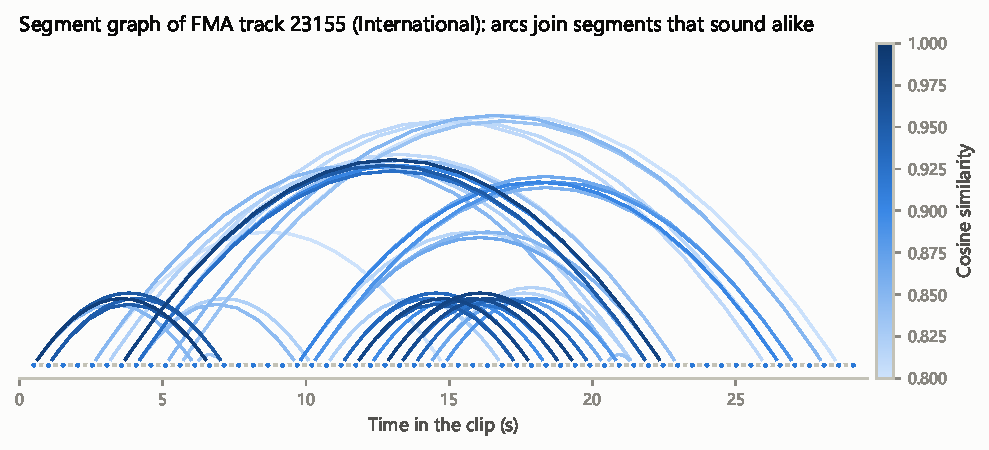
\includegraphics[width=\linewidth]{song_arc_diagram}
  \caption{A segment graph drawn as an arc diagram. Dots are one-second segments along the time axis, the grey line is
  the chain of temporal edges, and each arc is a similarity edge coloured by centred chroma cosine similarity. Long arcs
  join moments far apart in time that sound alike, which is how repetition appears to the GNN.}
  \label{fig:arc}
\end{figure}

% ------------------------------------------------------------------------------------------------
\section{Models}
\label{sec:models}

\begin{figure}[t]
  \centering
  \resizebox{\linewidth}{!}{%
  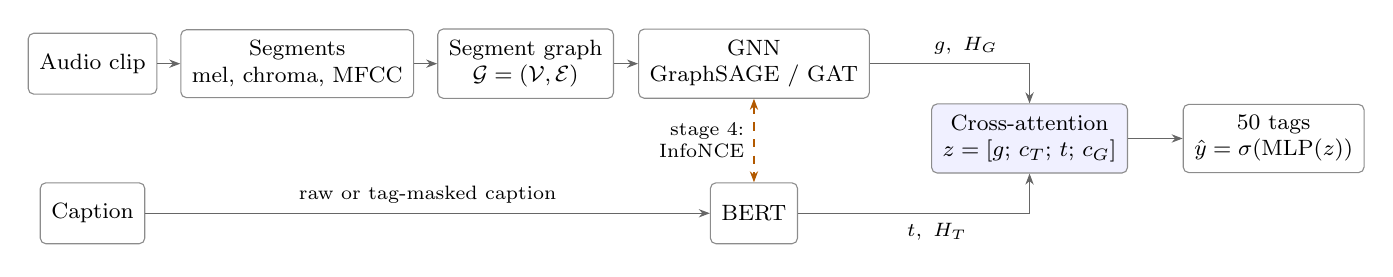
\begin{tikzpicture}[
      box/.style={draw=black!45, rounded corners=2pt, align=center, font=\footnotesize, inner sep=4pt, minimum height=2.2em},
      arrow/.style={-{Stealth[length=4pt]}, draw=black!60}]
    \node[box] (audio) at (0, 0) {Audio clip};
    \node[box] (seg) at (2.6, 0) {Segments\\mel, chroma, MFCC};
    \node[box] (graph) at (5.5, 0) {Segment graph\\$\mathcal{G}=(\mathcal{V},\mathcal{E})$};
    \node[box] (gnn) at (8.4, 0) {GNN\\GraphSAGE / GAT};
    \node[box] (text) at (0, -1.9) {Caption};
    \node[box] (bert) at (8.4, -1.9) {BERT};
    \node[box, fill=blue!6] (fuse) at (11.9, -0.95) {Cross-attention\\$z=[g;\,c_T;\,t;\,c_G]$};
    \node[box] (tags) at (15.0, -0.95) {50 tags\\$\hat y=\sigma(\mathrm{MLP}(z))$};
    \draw[arrow] (audio) -- (seg);
    \draw[arrow] (seg) -- (graph);
    \draw[arrow] (graph) -- (gnn);
    \draw[arrow] (text) -- node[above, font=\scriptsize] {raw or tag-masked caption} (bert);
    \draw[arrow] (gnn.east) -| node[pos=0.3, above, font=\scriptsize] {$g,\ H_G$} (fuse.north);
    \draw[arrow] (bert.east) -| node[pos=0.3, below, font=\scriptsize] {$t,\ H_T$} (fuse.south);
    \draw[arrow] (fuse) -- (tags);
    \draw[{Stealth[length=4pt]}-{Stealth[length=4pt]}, dashed, draw=orange!70!black] (gnn.south) --
      node[left, font=\scriptsize, align=right] {stage 4:\\InfoNCE} (bert.north);
  \end{tikzpicture}%
  }
  \caption{Leitmotif. Audio becomes a segment graph encoded by a GNN, and captions are encoded by BERT. Stage 3 fuses
  the two with bidirectional cross-attention to predict tags; stage 4 instead aligns the graph embedding $g$ and the
  caption vector $t$ in a shared space trained with InfoNCE.}
  \label{fig:architecture}
\end{figure}

\paragraph{Stage 1: BERT tagger.}
A caption $X$ is tokenised to at most 128 WordPiece tokens and encoded by \texttt{bert-base-uncased}. The final [CLS]
vector $t$ feeds one logistic output per tag, $\hat y_k = \sigma(w_k^\top t + b_k)$, trained with the mean binary
cross-entropy over the $K=50$ tags,
\begin{equation}
  \mathcal{L}_{\text{BERT}} = -\frac{1}{K}\sum_{k=1}^{K}\big[y_k \log \hat y_k + (1-y_k)\log(1-\hat y_k)\big].
\end{equation}

\paragraph{Stage 2: graph encoder.}
Node features are first projected to $d_G = 256$ dimensions, $h^{(0)}_i = W_0 x_i$, followed by three message-passing
layers, each with a residual connection and layer normalisation. The GraphSAGE layer uses mean aggregation,
\begin{equation}
  h_i^{(l+1)} = \mathrm{LN}\Big(h_i^{(l)} + \mathrm{Drop}\big(\mathrm{ReLU}\big(W_1^{(l)} h_i^{(l)} + W_2^{(l)}
  \tfrac{1}{|\mathcal{N}(i)|}\textstyle\sum_{j\in\mathcal{N}(i)} h_j^{(l)}\big)\big)\Big),
\end{equation}
where $W_1 h_i + W_2 \bar h_{\mathcal{N}(i)}$ equals $W\,[h_i \,;\, \bar h_{\mathcal{N}(i)}]$ from the brief with
$W = [W_1\; W_2]$. The GAT variant replaces the aggregation with four-head GATv2 attention that also sees the edge
attributes, $\alpha_{ij} = \operatorname{softmax}_j\big(a^\top \mathrm{LeakyReLU}(\Theta_s h_i + \Theta_t h_j + \Theta_e
e_{ij})\big)$ \citep{brody2022gatv2}. The graph embedding is the mean of the final node states,
$g = \frac{1}{|\mathcal{V}|}\sum_i h^{(L)}_i$. FMA genres are single-label, so the genre head is a softmax trained with
cross-entropy rather than the per-class sigmoid used for tags. We also test two variations. \emph{Crops}: each epoch,
every training graph is replaced by a random run of consecutive segments covering half the clip, the graph counterpart
of cropping a spectrogram in time, while evaluation uses whole clips. \emph{CNN node features}: a small CNN (three
blocks of $3\times3$ convolution with 16, 32 and 64 channels, batch normalisation, ReLU and $2\times2$ max pooling,
followed by global mean and max pooling and a linear layer) embeds each segment's $128\times43$ log-mel patch into 128
dimensions; the embedding is concatenated with $x_i$ before the input projection and trained end to end with the GNN.

\paragraph{CNN baseline.}
The spectrogram baseline is a VGG-style CNN with four blocks of two $3\times3$ convolutions (32, 64, 128 and 256
channels, batch normalisation, ReLU) and $2\times2$ max pooling, followed by global mean and max pooling, dropout and a
linear layer. It receives the full 128-band log-mel spectrogram and neither the graph nor any text.

\paragraph{Stage 3: fusion.}
Let $H_T \in \R^{L\times d}$ be BERT's token states projected to $d = 256$, with $t = H_T[\text{CLS}]$, and let
$H_G \in \R^{N\times d}$ be the projected node states of a clip, with projected graph embedding $g$. The
\emph{cross-attention} model builds
\begin{align}
  c_T &= \mathrm{MHA}\big(Q = g,\; K = V = H_T\big), &
  A &= \operatorname{softmax}\!\Big(\frac{(gW_Q)(H_TW_K)^\top}{\sqrt{d_h}}\Big), \\
  c_G &= \frac{1}{L}\sum_{l=1}^{L}\mathrm{MHA}\big(Q = H_T[l],\; K = V = H_G\big), &
  z &= [\,g \,;\, c_T \,;\, t \,;\, c_G\,] \in \R^{4d},
\end{align}
with four heads of size $d_h = 64$ and padding positions masked. The first term is the brief's graph-to-text attention.
The second runs from every caption token to the clip's segments; its attention matrix
$A^{T\to G} \in \R^{L\times N}$ shows which moments of the audio each word lines up with, which we use for the case
studies. A two-layer MLP maps $z$ to 50 tag logits trained with binary cross-entropy. The ablation replaces $z$ by $t$
(BERT only), $g$ (GNN only) or $[g\,;\,t]$ (early concatenation). In every variant the top four BERT layers are
fine-tuned and the rest stay frozen, and the graph encoder is the stage-2 GAT with CNN node features, initialised from
its FMA-small weights; stage 4 uses the same initialisation.

\paragraph{Stage 4: contrastive dual encoder.}
Two-layer projection heads map $g_i$ and $t_i$ to unit vectors $\hat g_i, \hat t_i \in \R^{256}$. With in-batch
negatives and a learnable temperature $\tau$ (initialised to 0.07, $1/\tau \le 100$), the symmetric InfoNCE loss
\citep{oord2018cpc, radford2021clip} over a batch of $N$ pairs is
\begin{equation}
  \mathcal{L}_{\text{NCE}} = -\frac{1}{2N}\sum_{i=1}^{N}\left[\log\frac{\exp(\hat g_i^\top \hat t_i/\tau)}
  {\sum_{j}\exp(\hat g_i^\top \hat t_j/\tau)} + \log\frac{\exp(\hat g_i^\top \hat t_i/\tau)}
  {\sum_{j}\exp(\hat g_j^\top \hat t_i/\tau)}\right].
\end{equation}
For zero-shot tagging, each tag $k$ is embedded as the normalised mean of the text embeddings of three prompts
(``\{tag\}'', ``this music is \{tag\}'', ``a recording featuring \{tag\}''), and clip $i$ receives the score
$\hat g_i^\top u_k$.

% ------------------------------------------------------------------------------------------------
\section{Experimental setup}
\label{sec:setup}

All models are trained with AdamW \citep{loshchilov2019adamw}, a linear warm-up over the first 10\% of steps (5\% for
models without BERT) followed by linear decay, bfloat16 mixed precision and gradient clipping at 1.0. Pretrained BERT
layers use a small learning rate and newly initialised layers a larger one; Appendix~\ref{app:hyper} lists every
hyperparameter. We keep the checkpoint with the best validation macro-F1 (mean recall for stage 4) and report test
results for that checkpoint only. For tag prediction, a single decision threshold is chosen on validation from
$\{0.05, 0.10, \dots, 0.95\}$ to maximise macro-F1 and then applied to the test set; per-epoch curves use 0.5. Training
ran on a single NVIDIA RTX 5060 Laptop GPU with 8\,GB of memory: a stage-1 epoch takes about 15\,s, a GNN epoch on
FMA-small 2--4\,s and a CNN epoch about 55\,s. The random seed is fixed at 42.

\paragraph{Metrics.}
For tags we report macro-F1 (the mean of per-tag F1), micro-F1 (F1 over all tag decisions pooled) and AUC-PR (the mean
over tags of average precision, skipping tags without positives in the split). For genre we report accuracy, macro-F1
and one-vs-rest AUC-PR. For retrieval we report recall at $K \in \{1, 5, 10\}$ and the median rank of the true match, in
both directions, over the whole test split.

\paragraph{Baselines.}
B1 guesses each tag at random with its training-set frequency (tags) or always predicts the most common training genre
(genre). B2 is the CNN on log-mel spectrograms. B3 is the BERT-only model of stage 1 and its audio-subset counterpart in
the stage-3 ablation.

% ------------------------------------------------------------------------------------------------
\section{Results}

\subsection{Stage 1: tags from text}
\label{sec:res-text}

Table~\ref{tab:text} shows that BERT is far above random guessing on both versions of the captions. Masking the tag
words costs 0.20 macro-F1 and 0.21 AUC-PR, which confirms that a large part of the raw-caption score comes from reading
labels directly off the text. The masked model still reaches 0.458 macro-F1, so the surrounding words (``it sounds like
something you would hear at Sunday services'') carry real context. Figure~\ref{fig:curves} shows that both runs converge
within ten epochs and that the gap between validation and test is larger in the masked setting.

\begin{table}[t]
  \caption{Stage 1, MusicCaps test split (2,858 captions, 50 tags). The threshold is chosen on validation.}
  \label{tab:text}
  \centering
  \small
  \begin{tabular}{lcccc}
    \toprule
    Model & Macro-F1 & Micro-F1 & AUC-PR & Threshold \\
    \midrule
    B1: random, tag frequency      & 0.078 & 0.125 & 0.078 & -- \\
    BERT, captions as written      & \textbf{0.659} & \textbf{0.720} & \textbf{0.680} & 0.40 \\
    BERT, tag words masked         & 0.458 & 0.569 & 0.471 & 0.30 \\
    \bottomrule
  \end{tabular}
\end{table}

\begin{figure}[t]
  \centering
  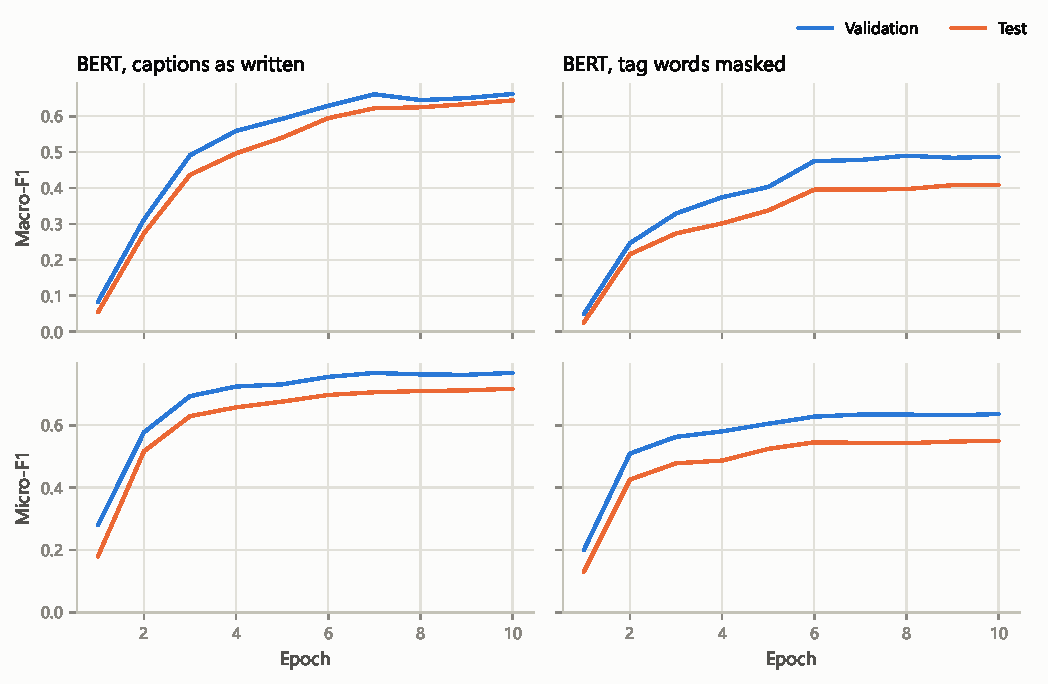
\includegraphics[width=0.85\linewidth]{stage1_curves}
  \caption{Stage 1 macro-F1 and micro-F1 by epoch at threshold 0.5, on raw (left) and masked (right) captions.}
  \label{fig:curves}
\end{figure}

\subsection{Stage 2: genre from structure}
\label{sec:res-graph}

\begin{table}[t]
  \caption{Stage 2, FMA-small test split (800 tracks, 8 balanced genres). ``+ crops'' trains on random half-length
  crops and evaluates on whole clips; ``+ CNN node features'' adds a learned embedding of each segment's log-mel patch
  to its node features.}
  \label{tab:graph}
  \centering
  \small
  \begin{tabular}{lccc}
    \toprule
    Model & Accuracy & Macro-F1 & AUC-PR \\
    \midrule
    B1: majority genre                 & 0.125 & 0.028 & 0.125 \\
    B2: CNN on log-mel                 & \textbf{0.541} & \textbf{0.537} & \textbf{0.572} \\
    \midrule
    GraphSAGE, chord graph             & 0.364 & 0.356 & 0.393 \\
    GAT, chord graph                   & 0.369 & 0.372 & 0.396 \\
    GraphSAGE, segment graph           & 0.384 & 0.379 & 0.403 \\
    GAT, segment graph                 & 0.396 & 0.400 & 0.411 \\
    GraphSAGE, segment graph + crops   & 0.374 & 0.369 & 0.375 \\
    GAT, segment graph + crops         & 0.378 & 0.378 & 0.388 \\
    \midrule
    GAT, segment graph + CNN node features & 0.484 & 0.485 & 0.514 \\
    \bottomrule
  \end{tabular}
\end{table}

All graph models are about three times as accurate as the majority baseline, and segment graphs beat chord graphs for
both encoders: the similarity structure of timbre and harmony over one-second windows says more about genre than a
sequence of template-matched triads, which are unreliable for genres such as Experimental or Hip-Hop that are not built
on chord progressions. GAT, which also sees the edge attributes, is slightly better than GraphSAGE on both graph types.
The CNN on full log-mel spectrograms is nevertheless clearly stronger, with 0.537 against 0.400 macro-F1. We attribute
most of the gap to the node features: each node summarises a second of audio by its mean spectrum, mean chroma and a
few MFCC statistics, which discards the fine time--frequency texture the CNN learns from. The graph models also
overfit, reaching near-zero training loss within 60 epochs while validation macro-F1 plateaus around 0.45, and training
on random half-length crops did not help them (0.369 and 0.378).

Giving the graph model that texture back closes most of the gap. When a small CNN embeds each segment's spectrogram
patch and GAT passes messages over the same segment graph, test macro-F1 rises from 0.400 to 0.485. The hybrid still
trails the CNN overall, but its errors differ (Figure~\ref{fig:confusion}): it recognises Electronic (recall 0.72 against
0.58 for the CNN) and Rock (0.56 against 0.50) better, while the CNN is well ahead on International (0.68 against
0.40) and Pop (0.52 against 0.33). One reading is that loop-based electronic music and riff-driven rock expose the
repetition the graph encodes, whereas International and Pop are told apart more by timbre and instrumentation across
the whole clip; we did not test this directly. Because it is the strongest graph encoder, the hybrid initialises the
graph side of stages 3 and 4.

\begin{figure}[t]
  \centering
  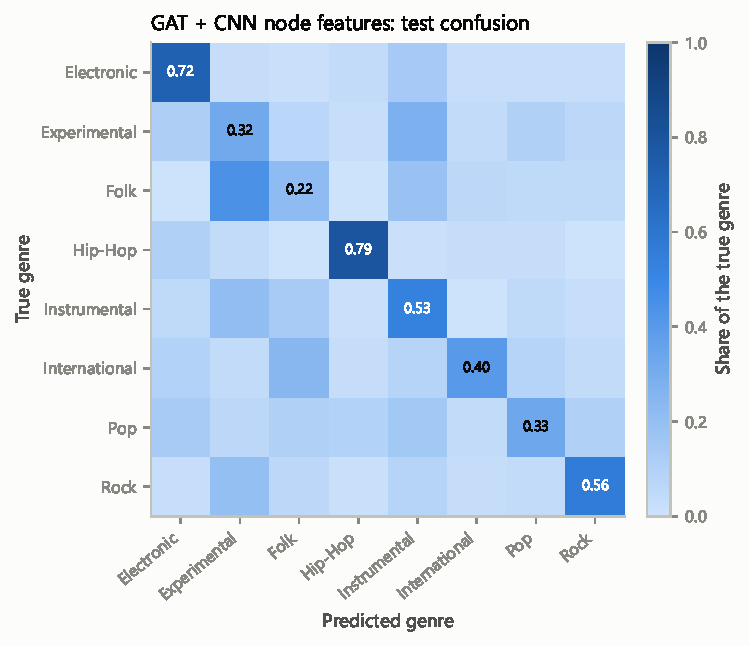
\includegraphics[width=0.55\linewidth]{stage2_confusion}
  \caption{Test confusion matrix of the best stage-2 graph model, normalised by true genre. Diagonal values are
  per-genre recall.}
  \label{fig:confusion}
\end{figure}

\subsection{Stage 3: fusing structure and text}
\label{sec:res-fusion}

\begin{table}[t]
  \caption{Stage 3 ablation on the MusicCaps test clips with audio, masked captions, 50 tags.}
  \label{tab:fusion}
  \centering
  \small
  \begin{tabular}{lccc}
    \toprule
    Fusion & Macro-F1 & Micro-F1 & AUC-PR \\
    \midrule
    GNN only (audio graph)           & \tbd{} & \tbd{} & \tbd{} \\
    BERT only (masked caption)       & \tbd{} & \tbd{} & \tbd{} \\
    Early concatenation $[g\,;\,t]$  & \tbd{} & \tbd{} & \tbd{} \\
    Cross-attention                  & \tbd{} & \tbd{} & \tbd{} \\
    \bottomrule
  \end{tabular}
\end{table}

\tbd{Discussion of Table~\ref{tab:fusion}, the t-SNE plot (Figure~\ref{fig:tsne}) and three case studies of
text-to-segment attention (Figure~\ref{fig:cases}).}

\begin{figure}[t]
  \centering
  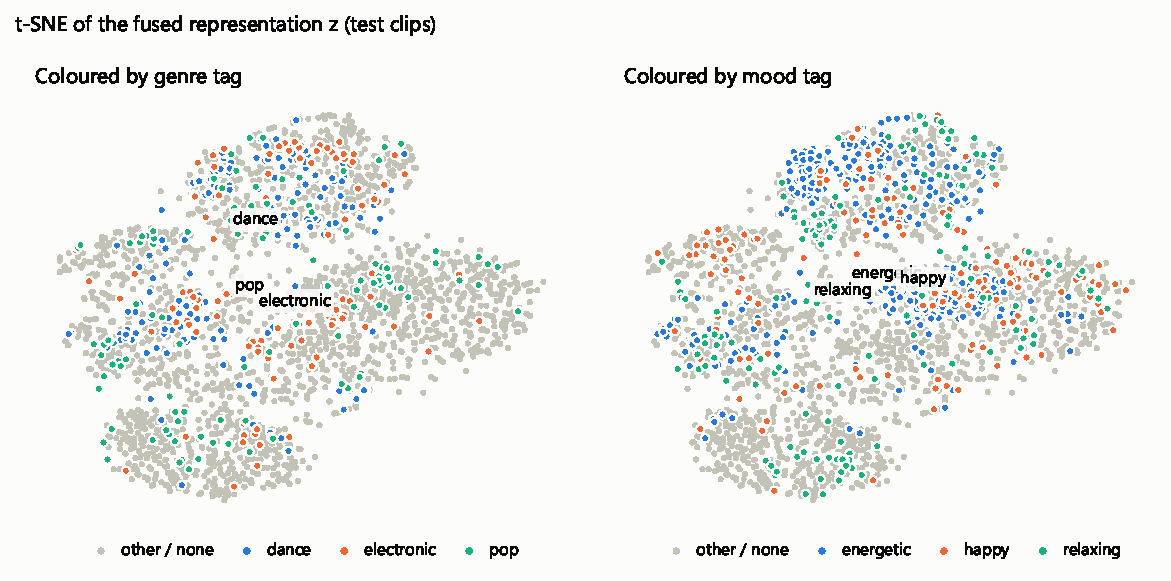
\includegraphics[width=\linewidth]{stage3_tsne}
  \caption{t-SNE of the fused representation $z$ for test clips, coloured by the most frequent genre tags (left) and
  mood tags (right). Clips with none of the three tags are grey.}
  \label{fig:tsne}
\end{figure}

\begin{figure}[t]
  \centering
  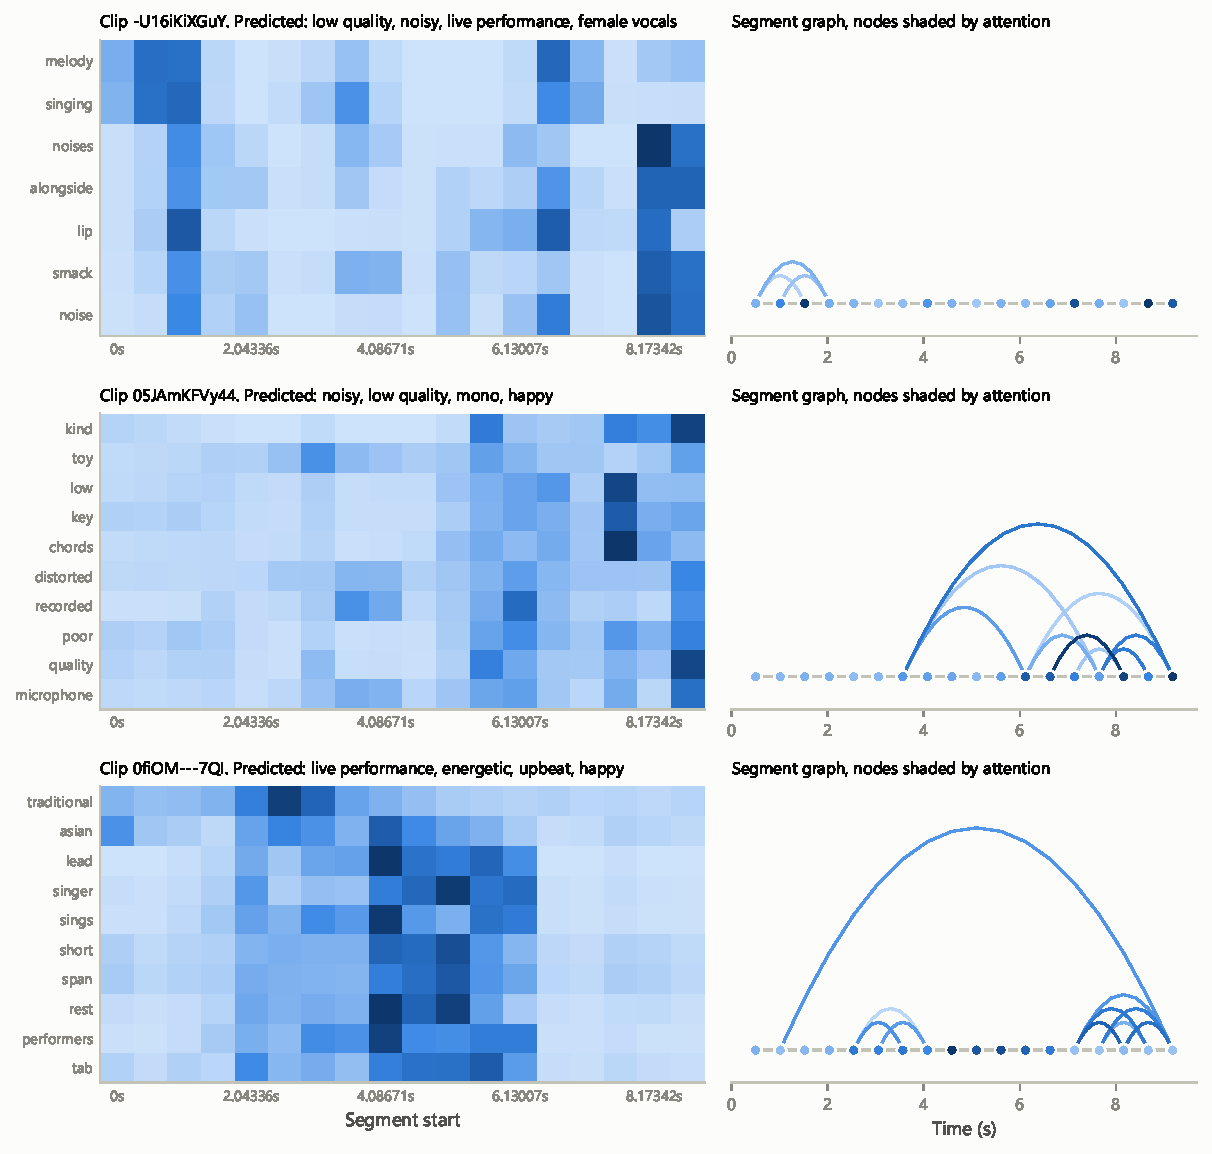
\includegraphics[width=\linewidth]{case_studies}
  \caption{Case studies. Left: caption words (rows) against one-second segments (columns) under the text-to-graph
  attention $A^{T\to G}$ of the cross-attention model. Right: the same clip's segment graph, with nodes shaded by the
  attention they receive averaged over the words shown.}
  \label{fig:cases}
\end{figure}

\subsection{Stage 4: text-to-music retrieval}
\label{sec:res-retrieval}

\begin{table}[t]
  \caption{Stage 4 retrieval over the \tbd{n} MusicCaps test clips with audio. Chance R@10 is \tbd{}.}
  \label{tab:retrieval}
  \centering
  \small
  \begin{tabular}{lcccc}
    \toprule
    Direction & R@1 & R@5 & R@10 & Median rank \\
    \midrule
    Caption $\to$ audio & \tbd{} & \tbd{} & \tbd{} & \tbd{} \\
    Audio $\to$ caption & \tbd{} & \tbd{} & \tbd{} & \tbd{} \\
    \bottomrule
  \end{tabular}
\end{table}

\tbd{Retrieval discussion, zero-shot AUC-PR against the stage-3 supervised model, and qualitative examples.}

\paragraph{Relevance of retrieved clips.}
The brief suggests rating retrieved clips with at least five human listeners. We did not run a listening study.
Instead, each of the 30 retrieved clips (10 caption queries, top 3 each) and three random clips per query are scored
on a 1--5 scale by three automatic judges that share no weights with our models: tag agreement ($1 + 4\times$ the
Jaccard overlap of the query clip's and candidate clip's tags), caption agreement (cosine similarity of the two
captions under the all-MiniLM-L6-v2 sentence encoder) and audio--text agreement (cosine similarity of the query caption
and the candidate's audio under the LAION CLAP model \texttt{clap-htsat-unfused}). The last two are expressed as
$1 + 4p$, where $p$ is the share of random test caption pairs, or caption--clip pairs, that score lower. \tbd{Scores.}
These scores are a proxy for, not a substitute for, human judgement; CLAP was pretrained on general audio--text data,
so it may share biases with our text encoder.

% ------------------------------------------------------------------------------------------------
\section{Discussion and limitations}

\tbd{Summarise what the graph view adds, when fusion helps, and the retrieval quality.}

\paragraph{Limitations.}
Captions and tags were written together, and masking removes only exact phrases. The labelled data is small: stages 3
and 4 train on at most 2,406 clips, and some MusicCaps videos are no longer available. Template-matched chords are a
coarse estimate of harmony. FMA genres are single-label, and FMA and MusicCaps differ in recording conditions, which
limits transfer of the pretrained graph encoder. Finally, retrieval quality is judged automatically rather than by
listeners.

\section{Conclusion}

\tbd{Conclusion.}

\paragraph{Reproducibility.}
The repository contains the full pipeline, from download scripts to training, evaluation and figures, with exact
dependency versions (\texttt{uv.lock}), the configuration used for every run (\texttt{config.yaml}), the data splits,
20 sample graphs in \texttt{.pt} and \texttt{.json} form, and an end-to-end inference notebook.

\bibliographystyle{plainnat}
\bibliography{references}

% ------------------------------------------------------------------------------------------------
\appendix

\section{Tag vocabulary}
\label{app:tags}

The 50 canonical tags, from most to least frequent on the training split: low quality, instrumental, bass, male
vocals, passionate, groovy, medium tempo, noisy, energetic, emotional, live performance, amateur recording, slow tempo,
fast tempo, electric guitar, mono, happy, piano, female vocals, acoustic drums, percussion, relaxing, shimmering
cymbals, punchy drums, keyboard, electronic drums, pop, acoustic guitar, classical, no other instruments, electronic,
dance, synth, upbeat, exciting, rock, eerie, romantic, strings, melodic, fun, sad, mellow, folk, easygoing, violin,
trumpet, soulful, claps, youthful. Examples of merged phrases: \emph{low quality} $\leftarrow$ poor audio quality, bad
audio quality, low quality recording; \emph{bass} $\leftarrow$ bass guitar, e-bass, groovy bass line; \emph{relaxing}
$\leftarrow$ calming, soothing, chill, meditative. The full table is in \texttt{src/tags.py}.

\section{Hyperparameters}
\label{app:hyper}

\begin{table}[h]
  \caption{Training settings. Learning rates are given as pretrained BERT layers / newly initialised layers; wd is
  the AdamW weight decay.}
  \centering
  \footnotesize
  \setlength{\tabcolsep}{4pt}
  \begin{tabular}{lcccl}
    \toprule
    Model & Epochs & Batch & Learning rate & Other settings \\
    \midrule
    Stage 1 BERT tagger  & 10 & 32 & $3{\times}10^{-5}$ / $10^{-3}$ & all layers tuned, max length 128, wd 0.01 \\
    Stage 2 GNN          & 60 & 64 & $10^{-3}$ & 3 layers, width 256, dropout 0.3, wd $10^{-4}$ \\
    Stage 2 + CNN nodes  & 20 & 32 & $10^{-3}$ & as above; patch CNN with 16/32/64 channels, 128-d embedding \\
    B2 CNN               & 30 & 32 & $10^{-3}$ & dropout 0.3, wd $10^{-4}$ \\
    Stage 3 fusion       & 15 & 32 & $2{\times}10^{-5}$ / $10^{-3}$ & $d{=}256$, 4 heads, top 4 BERT layers, wd 0.01 \\
    Stage 4 dual encoder & 30 & 64 & $2{\times}10^{-5}$ / $5{\times}10^{-4}$ & $\tau_0{=}0.07$, top 4 BERT layers, wd 0.01 \\
    \bottomrule
  \end{tabular}
\end{table}

\section{Additional figures}
\label{app:figures}

\begin{figure}[h]
  \centering
  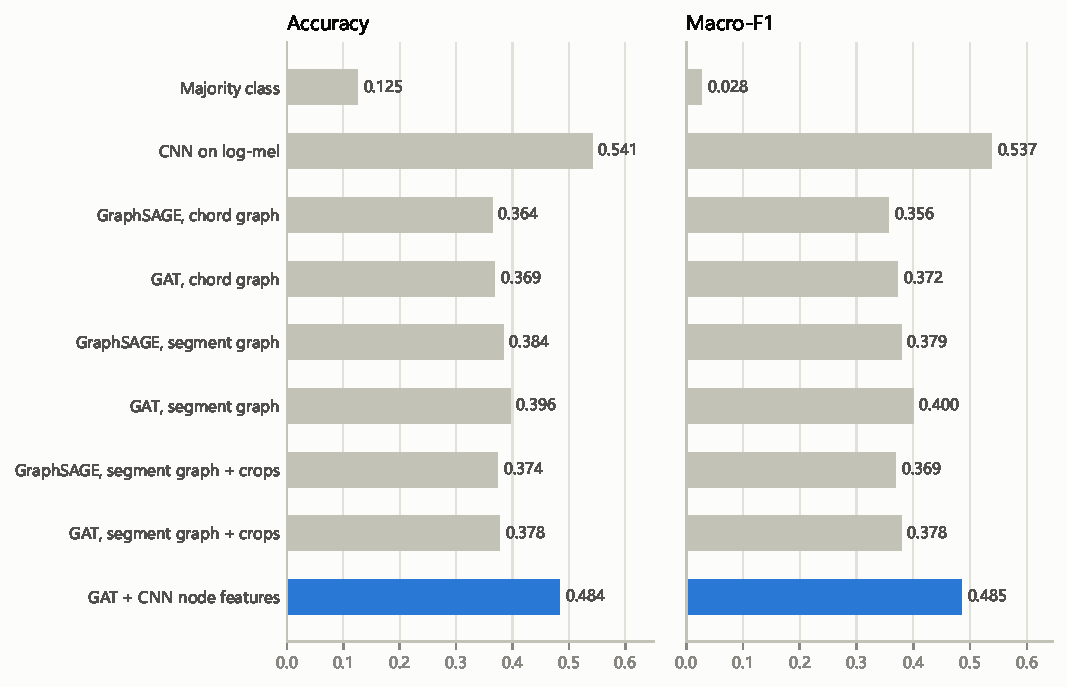
\includegraphics[width=0.9\linewidth]{stage2_comparison}
  \caption{Stage 2 test accuracy and macro-F1 on FMA-small. The best model that is not a baseline is blue; baselines
  and the other models are grey.}
  \label{fig:stage2-bars}
\end{figure}

\begin{figure}[h]
  \centering
  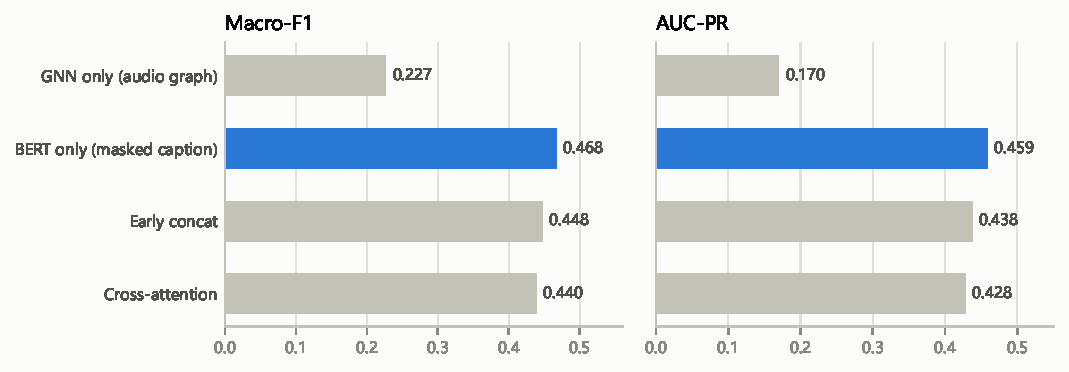
\includegraphics[width=0.9\linewidth]{stage3_ablation}
  \caption{Stage 3 ablation on masked captions: test macro-F1 and AUC-PR. The best fusion variant is blue.}
  \label{fig:stage3-bars}
\end{figure}

\begin{figure}[h]
  \centering
  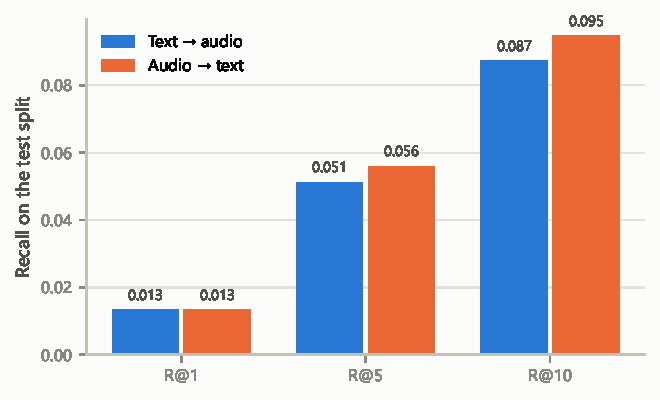
\includegraphics[width=0.6\linewidth]{stage4_retrieval}
  \caption{Stage 4 recall at $K$ over the MusicCaps test clips with audio, for caption-to-audio and audio-to-caption
  retrieval.}
  \label{fig:stage4-bars}
\end{figure}

\end{document}
